\documentclass[crop,tikz]{standalone}
\usepackage{tikz}

\usetikzlibrary{positioning}

\begin{document}
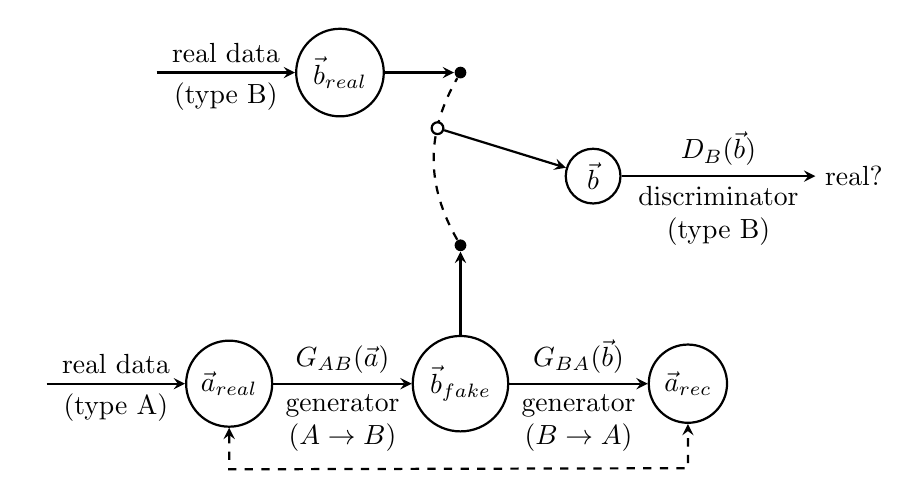
\begin{tikzpicture}
	\node[circle, draw, thick] (z) {$\vec{a}_{real}$};
	\node[circle, draw, thick, right=5em of z] (x) {$\vec{b}_{fake}$};
	\draw[-stealth, thick] (z) -- node[above] {$G_{AB}(\vec{a})$} node[below, align=center] {generator\\ ($A\rightarrow B$)} (x);
	\node[circle, draw, thick, right=5em of x] (xx) {$\vec{a}_{rec}$};
	\draw[-stealth, thick] (x) -- node[above] {$G_{BA}(\vec{b})$} node[below, align=center] {generator\\ ($B\rightarrow A$)} (xx);
	\node[left=5em of z] (i) {};
	\draw[-stealth, thick] (i) -- node[above] {real data} node[below] {(type A)} (z);

	\node[circle, draw, thick, right=2em of x, yshift=7.5em] (D) {$\vec{b}$};
	\node[right=7em of D] (out) {real?};
	\draw[-stealth, thick] (D) -- node[above] {$D_B(\vec{b})$} node[below,align=center] {discriminator\\ (type B)} (out);
		
	\node[yshift=5em, circle, fill, inner sep=0.15em] at (x) (pt1) {};
	\node[above=of x, yshift=6.4em, circle, fill, inner sep=0.15em] (pt2) {};

	\node[left=2.5em of pt2, circle, draw, thick] (xt) {$\vec{b}_{real}$};
	\node[left=5em of xt] (it) {};
	\draw[-stealth, thick] (it) -- node[above] {real data} node[below] {(type B)} (xt);

	\draw[dashed, thick] (pt1) edge[bend left] (pt2);

	\node[circle, draw, thick, fill=white, inner sep=0.15em] at ([xshift=-0.83em, yshift=4em]pt1.north) (pt3) {};

	\draw[-stealth, thick] (x) -- (pt1);
	\draw[-stealth, thick] (xt) -- (pt2);
	\draw[-stealth, thick] (pt3) -- (D);

	\draw[dashed, thick, stealth-stealth] (z.south) -- ([yshift=-1.5em]z.south) -- ([yshift=-1.6em]xx.south) -- (xx.south);
\end{tikzpicture}
\end{document}